\section{Organisation d'un document}

\begin{frame}[plain]
  \begin{conseil}
    Utilisez impérativement les commandes {\LaTeX} pour identifier
    les différentes parties (la structure) d'un document.
  \end{conseil}
\end{frame}

\subsection{Parties d'un document}

\begin{frame}[fragile]
  \frametitle{Titre et page de titre}
  \begin{itemize}
  \item Mise en forme automatique
    \begin{lstlisting}
%% préambule
\title{`\textit{Titre du document}'}
\author{`\textit{Prénom Nom}'}
\date{`\textit{31 octobre 2014}'} % automatique si omis

%% corps du document
\maketitle
    \end{lstlisting}
  \item Mise en forme libre \\[6pt]
    \begin{minipage}{0.45\linewidth}
      \begin{block}{\small classes standards}
\begin{lstlisting}
\begin{titlepage}
  ...
\end{titlepage}
\end{lstlisting}
      \end{block}
    \end{minipage}
    \hfill
    \begin{minipage}{0.45\linewidth}
      \begin{block}{\small classe \class{memoir}}
\begin{lstlisting}
\begin{titlingpage}
  ...
\end{titlingpage}
\end{lstlisting}
      \end{block}
    \end{minipage}
  \end{itemize}
\end{frame}

\begin{frame}[fragile=singleslide]
  \frametitle{Résumé}
  \begin{itemize}
  \item Classes \class{article}, \class{report} ou \class{memoir}:
    résumé créé avec l'environnement
\begin{lstlisting}
\begin{abstract}

\end{abstract}
\end{lstlisting}
  \item Classe \class{ulthese}: résumés français et anglais traités
    comme des chapitres normaux (non numérotés)
  \end{itemize}
\end{frame}

\begin{frame}[fragile=singleslide]
  \frametitle{Sections}
  \begin{itemize}
  \item Découpage du document en sections avec les commandes
\begin{lstlisting}
\part{`\textit{titre}'}
\chapter{`\textit{titre}'}
\section{`\textit{titre}'}
\subsection{`\textit{titre}'}
\end{lstlisting}
\begin{lstlisting}
\subsubsection{`\textit{titre}'}     % à éviter dans un livre
\end{lstlisting}
\begin{lstlisting}
\paragraph{`\textit{titre}'}         % jamais (?) utilisé
\subparagraph{`\textit{titre}'}      % idem
\end{lstlisting}
  \item Numérotation automatique
  \item Commande suivie d'une \verb=*= = section non numérotée
  \item Titre «court» en argument optionnel
  \end{itemize}
\end{frame}

\begin{frame}[fragile=singleslide]
  \frametitle{Annexes}
  \begin{itemize}
  \item Les annexes sont des sections ou des chapitres avec une numérotation
    alphanumérique (A, A.1, ...)
  \item Sections suivantes identifiées comme des annexes par la
    commande
\begin{lstlisting}
\appendix
\end{lstlisting}
  \item Dans le titre, «Chapitre» changé pour «Annexe» le cas échéant
  \end{itemize}
\end{frame}

\begin{frame}[fragile]
  \frametitle{Structure logique d'un livre}
  \framesubtitle{(classes \class{book}, \class{memoir}, \class{ulthese})}
\begin{lstlisting}
\frontmatter
\end{lstlisting}
  \begin{itemize}
    \small
  \item préface, table des matières, etc.
  \item numérotation des pages en chiffres romains (i, ii, ...)
  \item chapitres non numérotés
  \end{itemize}
  \vfill

\begin{lstlisting}
\mainmatter
\end{lstlisting}
  \begin{itemize}
    \small
  \item le contenu à proprement parler
  \item numérotation des pages à partir de 1 en chiffres arabes
  \item chapitres numérotés
  \end{itemize}
  \vfill

\begin{lstlisting}
\backmatter
\end{lstlisting}
  \begin{itemize}
    \small
  \item tout le reste (bibliographie, index, etc.)
  \item numérotation des pages se poursuit
  \item chapitres non numérotés
  \end{itemize}
\end{frame}

\subsection{Table des matières}

\begin{frame}[fragile]
  \frametitle{Table des matières}
  \begin{itemize}
  \item Table des matières produite automatiquement avec
\begin{lstlisting}
\tableofcontents
\end{lstlisting}
  \item Requiert plusieurs compilations
  \item Sections non numérotées pas incluses
  \item Avec \pkg{hyperref}, produit également la table des
    matières du fichier PDF
  \item<2-> Classe \class{memoir} fournit également
\begin{lstlisting}
\tableofcontents*
\end{lstlisting}
    qui n'insère pas la table des matières dans la table des matières
  \item<3-> Aussi disponibles:
\begin{lstlisting}
\listoffigures
\listoftables
\end{lstlisting}
    (et leurs versions \verb=*= dans \class{memoir})
  \end{itemize}
\end{frame}

%%% >>>
\stepcounter{exerciceref}
\subsection{[~Exercice \theexerciceref~]}

\begin{frame}[fragile=singleslide,plain]
  \begin{exercice}
    Utiliser le fichier \fichier{exercice\_parties.tex}.
    \begin{enumerate}
    \item Étudier la structure du document dans le code source.
    \item Ajouter un titre et un auteur au document.
    \item Créer la table des matières du document en le compilant 2 à
      3 fois.
    \item Insérer deux ou trois titres de sections de différents niveaux
      dans le document.
    \item Vous remarquerez que la numérotation cesse à partir des
      sous-sections. C'est une particularité de la classe
      \class{memoir}.

      Recompiler le document après avoir ajouté au préambule la commande
\begin{lstlisting}
\maxsecnumdepth{subsection}
\end{lstlisting}
    \item Ajouter une annexe au document.
    \end{enumerate}
  \end{exercice}
\end{frame}
%%% <<<

\subsection{Renvois automatiques}

\begin{frame}[fragile=singleslide]
  \frametitle{Étiquettes et renvois automatiques}
  \framesubtitle{Parce que l'ordinateur le fera mieux que vous}

  \begin{itemize}
  \item Ne \alert{jamais} renvoyer manuellement à un numéro de
    section, d'équation, de tableau, etc.
  \item «Nommer» un élément avec \verb=\label=
  \item Faire référence par son nom avec \verb=\ref=
  \item Requiert 2 à 3 compilations
  \end{itemize}
\end{frame}

\begin{frame}[plain,fragile=singleslide]
  \begin{lstlisting}[emph={\label,\ref}]
\section{Définitions}
\label{sec:definitions}

Lorem ipsum dolor sit amet, consectetur
adipiscing elit. Duis in auctor dui. Vestibulum
ut, placerat ac, adipiscing vitae, felis.

\section{Historique}

Tel que vu à la section \ref{sec:definitions},
on a...
\end{lstlisting}
  \fbox{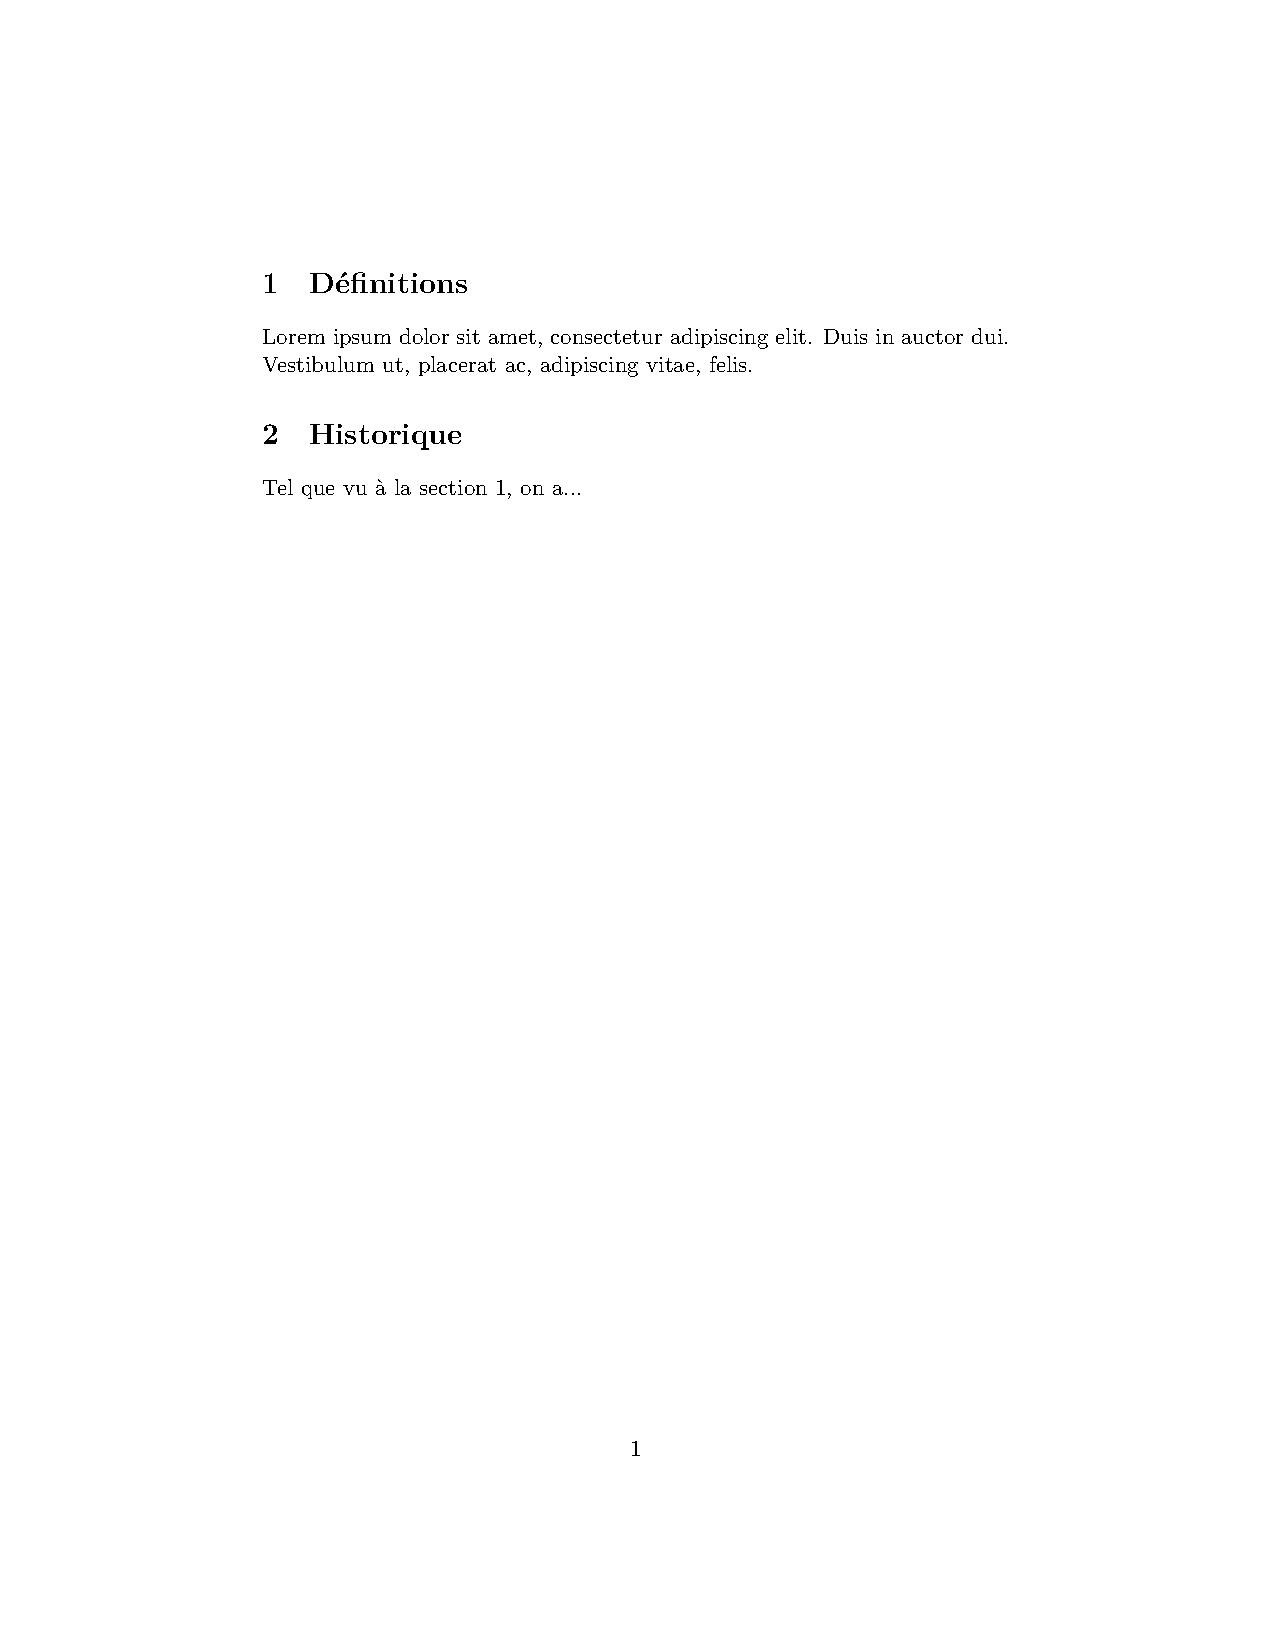
\includegraphics[viewport=124 550 484 664,clip=true,width=0.98\linewidth]{exemple-renvoi}}
\end{frame}

\begin{frame}[plain,fragile=singleslide]
  \begin{conseil}
    Adoptez une manière systématique et mnémotechnique de nommer les
    éléments dans un long document afin de vous y retrouver.

    \bigskip %
    Exemple:
\begin{lstlisting}
\label{chap:`\textit{chapitre}'}         % chapitre
\label{sec:`\textit{chapitre}':`\textit{section}'}  % section
\label{tab:`\textit{chapitre}':`\textit{tableau}'}  % tableau
\label{eq:`\textit{chapitre}':`\textit{equation}'}  % équation
\end{lstlisting}
  \end{conseil}
\end{frame}

\subsection{Hyperliens}

\begin{frame}[fragile]
  \frametitle{Renvois automatiques++}
  \begin{itemize}
  \item Paquetage \pkg{hyperref} insère des hyperliens vers les
    renvois dans les fichiers PDF
\begin{lstlisting}
Tel que vu à la section \ref{sec:definitions},
on a...
\end{lstlisting}
    \fbox{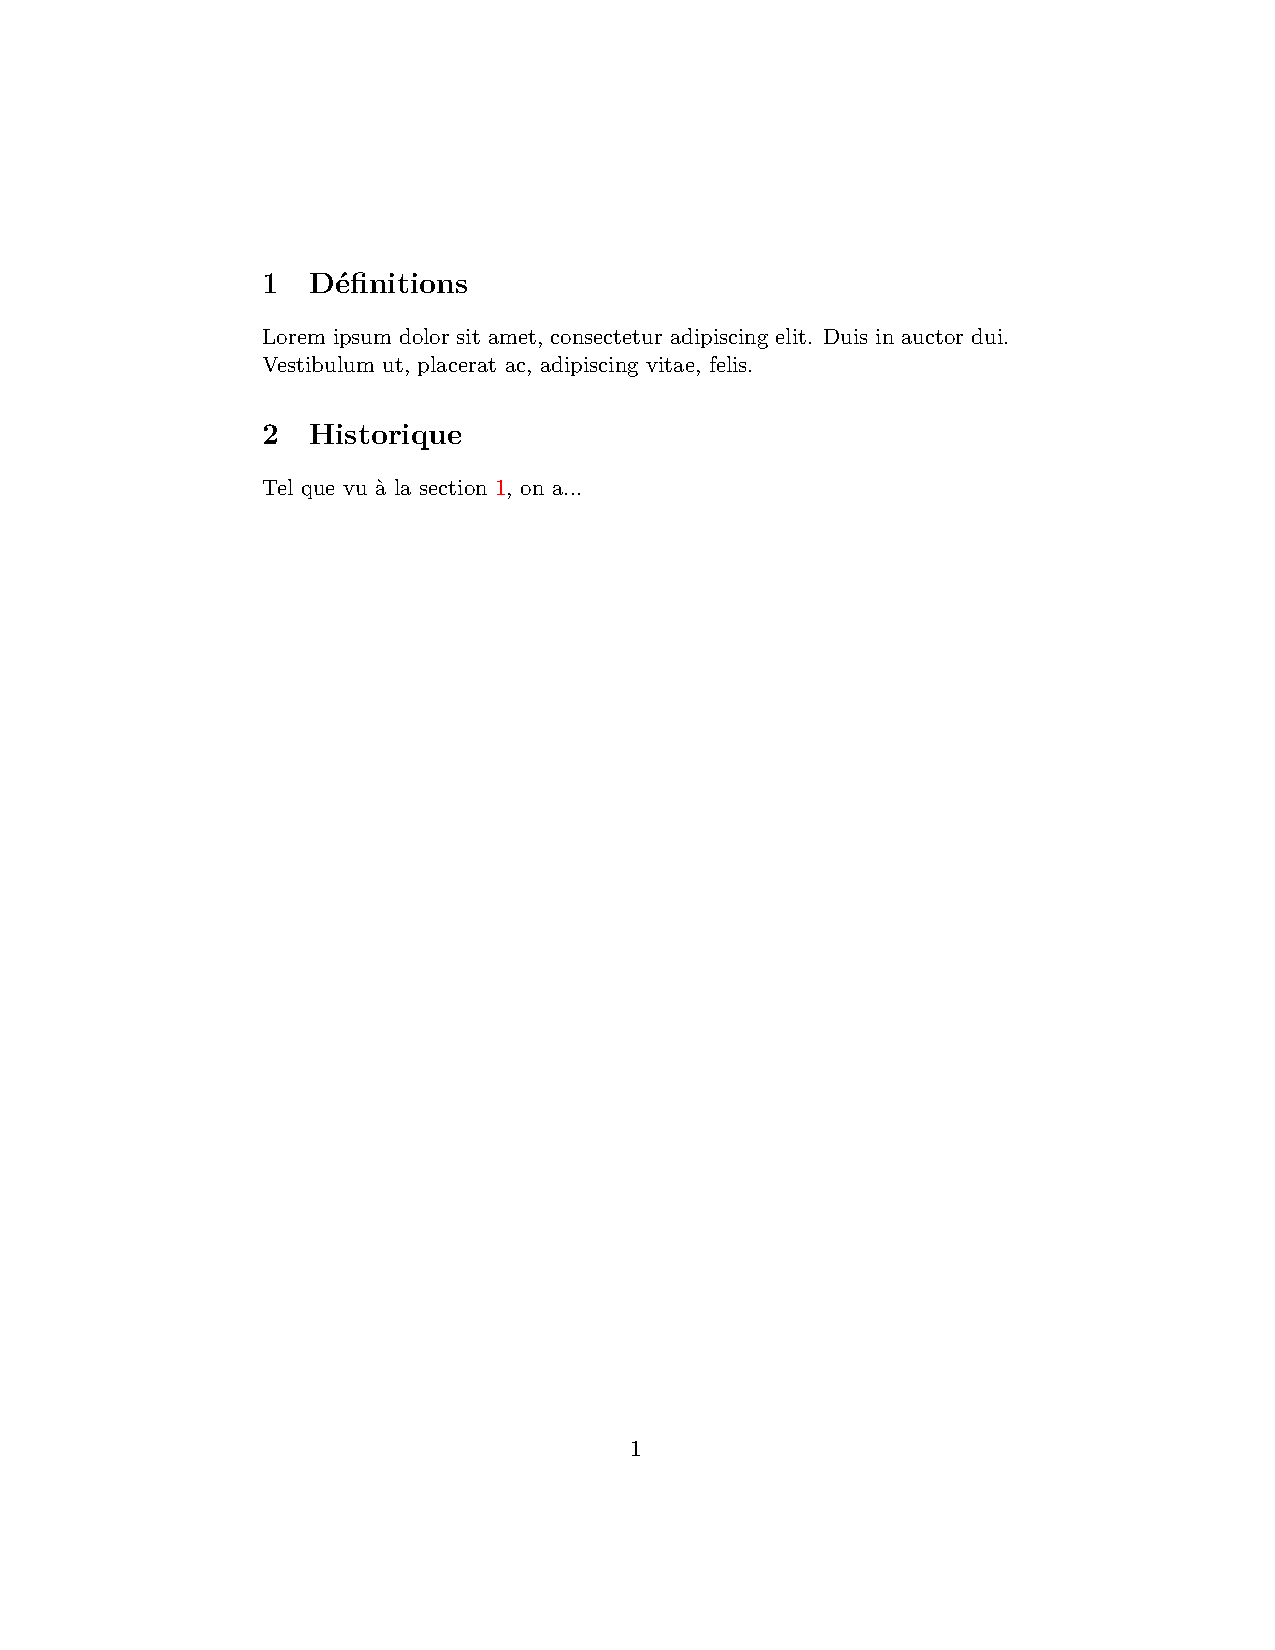
\includegraphics[viewport=124 550 484 564,clip=true,width=0.98\linewidth]{exemple-renvoi-hyperref}}
    \vfill
  \item<2-> Commande \verb=\autoref= permet de
    \begin{enumerate}
    \item nommer automatiquement le type de renvoi (section, équation,
      tableau, etc.)
    \item transformer en hyperlien le texte \textbf{et} le numéro
    \end{enumerate}
\begin{lstlisting}
Tel que vu à la \autoref{sec:definitions},
on a...
\end{lstlisting}
    \fbox{\includegraphics[viewport=124 550 484 564,clip=true,width=0.98\linewidth]{exemple-renvoi-autoref}}
  \end{itemize}
\end{frame}

%%% >>>
\stepcounter{exerciceref}
\subsection{[~Exercice \theexerciceref~]}

\begin{frame}[plain]
  \begin{exercice}
    Utiliser le fichier \fichier{exercice\_renvois.tex}.
    \begin{enumerate}
    \item Insérer dans le texte un renvoi au numéro d'une section.
    \item Activer le paquetage \pkg{hyperref} avec l'option
      \texttt{colorlinks} et comparer l'effet d'utiliser
      \texttt{{\textbackslash}ref} ou \texttt{{\textbackslash}autoref}
      pour le renvoi.
    \end{enumerate}
  \end{exercice}
\end{frame}
%%% <<<

%%% Local Variables:
%%% mode: latex
%%% TeX-engine: xetex
%%% TeX-master: "formation-latex-ul-diapos"
%%% End:
